\chapter{Authentifizierung}
\begin{itemize}
	\item \textbf{Authentifizierung:} Nachweis der \textit{Identität} eines Subjektes gegenüber einem anderen
	\item \textbf{Verifikation:} Identität wird bestätigt.
	\item \textbf{Identifikation:} Finden und Identifizieren eines Subjektes anhand von Referenzdaten (Fingerabdruck, Bild, ...)
\end{itemize}

\section{Voraussetzung für Authentifizierung}
\paragraph{Identifikationsmittel}
\begin{itemize}
	\item muss \textbf{eindeutig} sein
	\item kann \textbf{öffentlich} bekannt sein
\end{itemize}

\paragraph{Beweismittel}
\begin{itemize}
	\item meist unter Verschluss
	\item Beispiele: Passwort, private key, Fingerabdruck, preshared key, Iris, Chipkarte
\end{itemize}

\section{Realisierung der Authentifizierung}

\paragraph{Wissen}
\begin{itemize}
	\item Passwort
	\item PSK, SSH-Private-Key
	\item \textbf{Einfach anzugreifen}
	\item \textbf{Einfach zu ändern}
\end{itemize}

\paragraph{Besitz}
\begin{itemize}
	\item SmartCard
	\item Schlüssel
	\item \textbf{Kann entzogen werden!}
\end{itemize}
$\Rightarrow$ \textbf{Nicht (einfach) zu kopieren!}

\paragraph{Eigenschaften}
\begin{itemize}
	\item Biometrisches Merkmal einer Person (Iris, Fingerabdruck)
	\item False acceptence/reject
\end{itemize}
$\Rightarrow$ \textbf{nicht revozierbar!}

\subsection{Multi-Faktor-Authentifizierung}
Kombination von \textbf{min. 2} verschiedenen Beweismitteln \textbf{unterschiedlicher} Kategorien.\\
$\Rightarrow$ \textbf{Kompromittierung eines Faktors reicht nicht aus!}

\section{Ergebnis der Authentifizierung}
Das Subjekt erhält \textbf{Authentifizierungsbeweis}:
\begin{itemize}
	\item Session Cookie (Webbrowser)
	\item Session Key (TLS)
	\item Shell (Linux)
\end{itemize}
$\Rightarrow$ Identität wird auf \textbf{rechnerinternes} Objekt abgebildet.\\
$\Rightarrow$ \textbf{Schutz} des Authentifizierungsbeweises ist notwendig!

\section{Anforderungen an Authentifizierung}
\paragraph{Allgemeine Anforderungen}
\begin{itemize}
	\item Schutz des Authentifizierungsbeweises
	\item Schutz des Beweismittels
	\item Ergonomisch
	\item Einfach zu administrieren
\end{itemize}

\paragraph{Anforderungen bei Netzwerkauthentifizierung}
\begin{itemize}
	\item Keine sensiblen Daten über das Netz, im Klartext!
	\item Verhindern von Replay-Attacken!
	\item Verhindern von Man-in-the-Middle Angriffen!
\end{itemize}

\section{Authentifizierung mit Passwort}
\begin{itemize}
	\item idR. wird das Passwort im Rechner als \textbf{Hash} hinterlegt.
	\textbf{Salted Hash:} Passwort wird um Salt ergänzt, gehashed und mit dem hinterlegtem Wert verglichen.
	\item Salt:
	\begin{itemize}
	\item \textbf{Zufällige}, \textbf{pro Eintrag individuelle} Zeichensequenz
	\item Verhindert, dass identische Passwörter mit identischen Hashes abgespeichert werden
	\item Erschwert Wörterbuch- und Rainbowtable-Angriffe
	\end{itemize}
\end{itemize}

\section{Angriffe auf Passwortauthentisierung}
\paragraph{Angriffe}
\begin{itemize}
	\item Wörterbuchattacken
	\item Wörterbuchattacken auf Hashes
	\item Rainbow-Tables
\end{itemize}

\paragraph{Gegenmaßnahmen}
\begin{itemize}
	\item Langsame Hash-Algorithmen verwenden
	\item Salt
	\item Schutz der Hashes vor Auslesen
	\item Automatisches Sperren der Authentifizierung nach definierter Anzahl von Fehlversuchen
	\item Multifaktor-Authentifizierung 
\end{itemize}

\section{Biometrische Authentifizierung}
\begin{itemize}
	\item verwendet \textbf{individuelle Körpermerkmale} (Fingerabdruck, Irismuster, etc)
	\item Wesentliches Merkmal: biometrische Eigenschaften sind \textbf{immer leicht unterschiedlich}
\end{itemize}
\textbf{Ablauf:}
\begin{itemize}
	\item Einlernphase: mehrere Datenproben werden entnommen, daraus \textbf{Referenzdaten} erstellt
	\item 	Authentifizierung: neue Datenprobe wird genommen und mit Referenzdaten verglichen.\\ \textbf{Genügend Ähnlichkeit} $\Rightarrow$ authentifiziert.
\end{itemize}

\subsection{False-Reject vs. False-Accept}
\begin{figure}[H]
	\begin{center}
		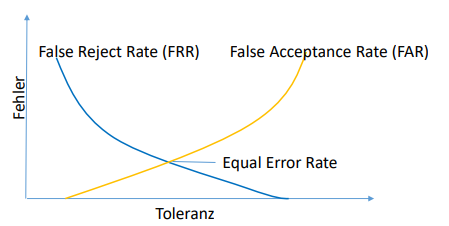
\includegraphics[scale=0.8]{Resources/FalseRejectFalseAcceptance.PNG}
		\caption{}
		\label{fig:FalseRejectFalseAcceptance.PNG}
	\end{center}
\end{figure}
\paragraph{False Reject Rate (FRR)}
\begin{itemize}
	\item Anteil der fälschlicherweise fehlgeschlagenen Authentifizierungsversuche
	\item Hohe FFR verringert Akzeptanz des Systems
\end{itemize}

\paragraph{False Acceptance Rate (FAR)}
\begin{itemize}
	\item Anteil der erfolgreichen
Authentifizierungsversuche, bei denen
fälschlicherweise eine andere Person
akzeptiert wird
	\item Hohe FAR verringert die Sicherheit deutlich!
\end{itemize}

\paragraph{Equal Error Rate}
\begin{itemize}
	\item Gibt die Toleranzschwelle an, bei der genauso viele Personen fälschlicherweise abgelehnt wie
fälschlicherweise akzeptiert werden (FAR=FRR)
	\item ist ein \textbf{Gütekriterium} für das biometrische Verfahren
	\item ist \textbf{nicht die Toleranzschwelle} mit der das System betrieben wird (normalerweise gilt: \textbf{FAR < FRR})
\end{itemize}

\section{Authentifizierung über Netzwerke}
\paragraph{zu Verhindern:}
\begin{itemize}
	\item Abhören
	\item Replay
	\item Man-in-the-Middle
	\item Übernehmen der authentifizierten Verbindung
	\item Ausfall des Authentifizierungssystems
\end{itemize}

\paragraph{Erreicht wird dies durch..}
\begin{itemize}
	\item Authentifizierung per Passwort (aber Verschlüsselte Verbindung)
	\item Zeitabhängige Passwörter / Einmalpasswörter
	\item Challenge-Response Authentifizierung
	\item Zertifikats- bzw. Public/Private-Key-Authentifizierung
\end{itemize}

\section{Einmalpasswörter}
Passwörter werden durch \textbf{Zähler} oder basierend \textbf{Zeitstempel} generiert.
Client und Server teilen gemeinsamen Schlüssel $K_A$ (individuell pro Client).
Der Schlüsselwert wird verwendet um:
\begin{itemize}
	\item aus einem Zählerwert $C$ und $K_A$ das Einmalpasswort zu bestimmen.
	\item aus dem aktuellen Zeitstempel $T$ und $K_A$ das Einmalpasswort zu bestimmen.
\end{itemize}
Server und Client berechnen unabhängig voneinander das Einmalpasswort. Die Authentifizierung ist erfolgreich, wenn dass Einmalpasswort übereinstimmt.\\
\\
\paragraph{Vorteile:}
\begin{itemize}
	\item Abgefangene Passwörter sind wertlos
	\item gemeinsamer Schlüssel $K_A$ kann clientseitig auf auslese-sicherer Hardware hinterlegt werden.
	\item Server erkennt Replay-Attacken
\end{itemize}
\paragraph{Nachteile:}
\begin{itemize}
	\item Gemeinsamer Schlüssel $K_A$ muss sicher auf Client und Server hinterlegt werden
	\item Ist $K_A$ bekannt können Einmalpasswörter vorrausberechnet werden. 
	\item Server hat Liste aller gemeinsamer Schlüssel
	\item Anfällig gegenüber Man-in-the-Middle.
	\begin{itemize}
		\item Separater Schutz gegen MiM notwendig!
		\item Typisch: Public-Private-Key-Auth des Server mittels SSL-Zertifikaten
	\end{itemize}
\end{itemize}

\section{Challenge-Response-Authentifizierung}
\begin{figure}[H]
	\begin{center}
		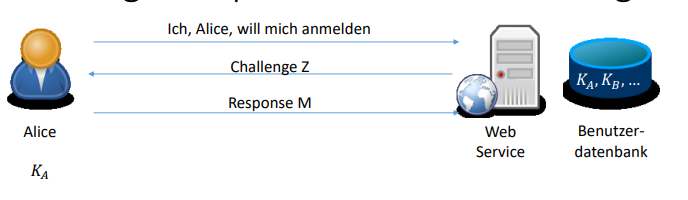
\includegraphics[scale=0.8]{Resources/ChallengeResponseAuth.png}
		\caption{}
		\label{fig:ChallengeResponeAuth.png}
	\end{center}
\end{figure}

\begin{enumerate}
	\item Alice schickt ihren Namen an den Server
	\item Server antwortet mit einer Nonce $Z$ (\enquote{Number used once}) an Alice
	\item Alice berechnet und schickt $M = Hash(K_A, Z)$ an den Server
	\item Server berechnet $M' = Hash(K_A, Z)$, falls $M' = M$ dann ist Alice authentifiziert.
	\item Alice und Server erzeugen gemeinsamen Session Key $K_S = KDF(K_A, Z)$
	\item Weitere Kommunikation wird mit $K_S$ verschlüsselt. $K_S$ ist der Authentifizierungsbeweis.
\end{enumerate}












